\documentclass[11pt]{article}
\usepackage[letterpaper,margin=2cm]{geometry}
\usepackage[english]{babel}
\usepackage[utf8]{inputenc}
\usepackage[T1]{fontenc}
\linespread{1.3}
\parskip=12pt
\parindent=0pt
\usepackage{enumerate}
\usepackage{amsmath}
\usepackage{amsfonts}
\usepackage{graphicx}
\usepackage[section]{placeins}
\usepackage{amsthm}
\usepackage{amssymb}
\usepackage{mathpazo}
\usepackage{booktabs}
\usepackage{float}
\usepackage{listings}

\usepackage[dvipsnames]{xcolor}
\definecolor{slateblue}{RGB}{45, 62, 80}
\definecolor{FGVBlue}{RGB}{0, 114, 188}
\usepackage{hyperref}
\hypersetup{
	colorlinks=true,
	linkcolor=FGVBlue,
	urlcolor=FGVBlue,
	citecolor=FGVBlue,
}

\lstset{language=R, basicstyle=\ttfamily\footnotesize, breaklines=true,
	commentstyle=\color{gray}, keywordstyle=\color{slateblue}\bfseries,
	frame=single, rulecolor=\color{lightgray}, columns=fullflexible, keepspaces=true}

% Custom commands
\newcommand{\E}{\mathbb{E}}
\newcommand{\Var}{\mathrm{Var}}
\newcommand{\Prob}{\mathbb{P}}
\newcommand{\symbf}[1]{\boldsymbol{#1}}

\theoremstyle{plain}
\newtheorem{proposition}{Proposition}
\renewcommand{\theproposition}{A.\arabic{proposition}}
\newtheorem{lemma}[proposition]{Lemma}
\newtheorem*{nmtheorem}{Theorem (Newey and McFadden, 1994, Theorem 2.7)}

\newcounter{problem}
\renewcommand{\theproblem}{\arabic{problem}}
\newcommand{\problem}{
	\stepcounter{problem}
	\section*{Problem \theproblem}
}
\newcommand{\itm}[1]{\par\textbf{#1)}\ }

\begin{document}
	\begin{center}
		{\LARGE{\textbf{Problem Set I -- Solutions}}}\\
		\vspace{0.2cm}
		Econometrics I - \textcolor{FGVBlue}{FGV EPGE}\\
		Instructor: Raul Guarini Riva \\
		TA: Taric Latif Padovani
	\end{center}

The code for Problems 3, 5 and 6 is in R and is reproduced at the end of each problem. Simulations use \texttt{set.seed(2026)}, so the numbers below are exactly reproducible.

%=====================================================================
\problem

Throughout, $K$ is a symmetric density, so $K(u)\ge 0$, $\int K(u)\,du = 1$ and $K(u)=K(-u)$, with $R(K)=\int K^2(u)\,du<\infty$. The workhorse is the change of variables $u=(z-x)/h$:
\begin{equation}\label{eq:cv}
	\E\left[\frac1h K\!\left(\frac{X_i-x}{h}\right)\right] = \frac1h\int K\!\left(\frac{z-x}{h}\right) f(z)\,dz = \int K(u) f(x+hu)\,du .
\end{equation}

\itm{a}
Each term $K\big((X_i-x)/h\big)$ is nonnegative and $1/(nh)>0$, so $\hat f_n(x)\ge 0$. For the integral, use $u=(X_i-x)/h$ in each term, so $dx = -h\,du$ and the limits swap:
\[
\int_{-\infty}^{\infty} K\!\left(\frac{X_i-x}{h}\right)dx = h\int_{-\infty}^{\infty} K(u)\,du = h
\quad\Longrightarrow\quad
\int_{-\infty}^{\infty}\hat f_n(x)\,dx = \frac{1}{nh}\sum_{i=1}^n h = 1 .
\]
So $\hat f_n$ is itself a density, for every sample and every $n$.

\itm{b}
Since the $X_i$ are identically distributed, $\E[\hat f_n(x)]$ equals \eqref{eq:cv}. Using $\int K = 1$,
\[
\E[\hat f_n(x)] - f(x) = \int K(u)\big[f(x+hu)-f(x)\big]\,du .
\]
For each fixed $u$, $f(x+hu)\to f(x)$ as $h\to 0$, because $f$ is continuous at $x$. Let $M=\sup_z f(z)<\infty$. The integrand is bounded by $2M\,K(u)$, which is integrable. By dominated convergence (along any sequence $h\to 0$), the integral goes to zero:
\[
\E[\hat f_n(x)] = f(x) + o(1).
\]
Boundedness of $f$ is what lets us use kernels with unbounded support (such as the Gaussian): far-away points get little weight, and they cannot carry arbitrarily large density.

\itm{c}
By independence,
\[
\Var\big(\hat f_n(x)\big) = \frac1n\Var\!\left(\frac1h K\!\left(\frac{X_i-x}{h}\right)\right)
= \frac1n\,\E\!\left[\frac{1}{h^2}K^2\!\left(\frac{X_i-x}{h}\right)\right] - \frac1n\Big(\E[\hat f_n(x)]\Big)^2 .
\]
For the first term, the same change of variables gives
\[
\E\!\left[\frac{1}{h^2}K^2\!\left(\frac{X_i-x}{h}\right)\right] = \frac1h\int K^2(u)f(x+hu)\,du = \frac1h\Big(f(x)R(K) + o(1)\Big),
\]
where the last step is dominated convergence again, now with dominating function $M K^2(u)$, integrable because $R(K)<\infty$. For the second term, item b) gives $\big(\E[\hat f_n(x)]\big)^2 = (f(x)+o(1))^2 = O(1)$. Putting the two together,
\[
\Var\big(\hat f_n(x)\big) = \frac{f(x)R(K)}{nh} + o\!\left(\frac1{nh}\right) + O\!\left(\frac1n\right)
= \frac{f(x)R(K)}{nh} + o\!\left(\frac1{nh}\right),
\]
because $\frac{1/n}{1/(nh)} = h\to 0$, so $O(1/n)=o(1/(nh))$.

\itm{d}
The mean squared error splits into variance plus squared bias:
\[
\E\Big[\big(\hat f_n(x)-f(x)\big)^2\Big] = \Var\big(\hat f_n(x)\big) + \Big(\E[\hat f_n(x)]-f(x)\Big)^2
= \underbrace{\frac{f(x)R(K)}{nh} + o\!\left(\frac1{nh}\right)}_{\to 0 \text{ since } nh\to\infty} + \underbrace{o(1)}_{\text{since } h\to 0}\ \longrightarrow\ 0 .
\]
By Markov's (Chebyshev's) inequality, for any $\varepsilon>0$,
\[
\Prob\big(|\hat f_n(x)-f(x)|>\varepsilon\big) \le \frac{\E\big[(\hat f_n(x)-f(x))^2\big]}{\varepsilon^2}\ \longrightarrow\ 0,
\]
so $\hat f_n(x)\xrightarrow{p} f(x)$. Each condition does one job: $h\to 0$ kills the bias and $nh\to\infty$ kills the variance.

\itm{e}
Let
\[
r(t) \equiv f(x+t) - f(x) - f'(x)\,t - \tfrac12 f''(x)\,t^2 .
\]
By \eqref{eq:cv}, symmetry ($\int uK(u)\,du=0$) and unit variance ($\int u^2K(u)\,du=1$),
\[
\E[\hat f_n(x)] = \int K(u)\Big[f(x) + f'(x)hu + \tfrac12 f''(x)h^2u^2 + r(hu)\Big]du
= f(x) + \frac{h^2}{2}f''(x) + \int K(u)\,r(hu)\,du .
\]
It remains to show that $\int K(u)r(hu)\,du = o(h^2)$. Fix $\varepsilon>0$. Because $f''$ is continuous at $x$, there is a $\delta>0$ such that $f$ is twice differentiable on $(x-\delta,x+\delta)$ and $|f''(x+t)-f''(x)|\le\varepsilon$ whenever $|t|<\delta$. Split the integral at $|u|=\delta/h$.

\emph{Near $x$ ($|hu|<\delta$).} Taylor's theorem with the Lagrange remainder gives $f(x+t) = f(x)+f'(x)t+\frac12 f''(\xi)t^2$ for some $\xi$ between $x$ and $x+t$, so $|r(t)| = \frac12|f''(\xi)-f''(x)|\,t^2\le \frac{\varepsilon}{2}t^2$. Hence
\[
\left|\int_{|u|<\delta/h} K(u)\,r(hu)\,du\right| \le \frac{\varepsilon}{2}h^2\int u^2K(u)\,du = \frac{\varepsilon}{2}h^2 .
\]
\emph{Far from $x$ ($|u|\ge\delta/h$).} Here we only use $f\le M$: $|r(hu)|\le 2M + |f'(x)|h|u| + \frac12|f''(x)|h^2u^2$. On this region $1\le (h u/\delta)^2$ and $h|u|\le h^2u^2/\delta$, so
\[
\left|\int_{|u|\ge\delta/h} K(u)\,r(hu)\,du\right| \le h^2\left(\frac{2M}{\delta^2} + \frac{|f'(x)|}{\delta} + \frac{|f''(x)|}{2}\right)\int_{|u|\ge \delta/h}u^2K(u)\,du = o(h^2),
\]
since the tail of the convergent integral $\int u^2K(u)\,du$ goes to zero as $\delta/h\to\infty$.

Together, $\limsup_{h\to 0} h^{-2}\left|\int K(u)r(hu)\,du\right|\le \varepsilon/2$ for every $\varepsilon>0$, so the remainder is $o(h^2)$ and
\[
\E[\hat f_n(x)] = f(x) + \frac{h^2}{2}f''(x) + o(h^2).
\]

\itm{f}
The leading bias is $\frac{h^2}{2}f''(x)$, so its sign is the sign of the curvature of $f$ at $x$. The estimator replaces $f(x)$ by a weighted average of $f$ over a window of width about $h$ around $x$.
\begin{itemize}
	\item Where $f$ is locally convex ($f''(x)>0$, e.g.\ in the tails of a bell-shaped density or at a trough), the average of $f$ around $x$ is above $f(x)$: the bias is positive.
	\item Where $f$ is locally concave ($f''(x)<0$, e.g.\ at a mode), the average is below $f(x)$: the bias is negative. Kernel estimates flatten peaks and fill in valleys.
	\item At an inflection point ($f''(x)=0$) the leading bias vanishes, and the bias is of smaller order than $h^2$.
\end{itemize}
The slope $f'(x)$ plays no role, because a symmetric kernel puts equal weight on both sides of $x$, so a linear trend averages out. The bias grows with both $|f''(x)|$ and $h^2$. Problem 6 shows this bias at work.

%=====================================================================
\problem

\itm{a}
Stack the data as
\[
V = \begin{pmatrix} Y_1\\ \vdots\\ Y_n\end{pmatrix},\qquad
Z = \begin{pmatrix} 1 & X_1-x_0\\ \vdots & \vdots\\ 1 & X_n-x_0\end{pmatrix},\qquad
W = \mathrm{diag}\left(\frac{1}{K_h(X_1-x_0)},\ \dots,\ \frac{1}{K_h(X_n-x_0)}\right),
\]
and let $\theta=(\alpha,\beta)'$. Then $W^{-1}=\mathrm{diag}\big(K_h(X_i-x_0)\big)$ and the objective is
\[
S(\theta) = \sum_{i=1}^n K_h(X_i-x_0)\big[Y_i-\alpha-\beta(X_i-x_0)\big]^2 = (V-Z\theta)'W^{-1}(V-Z\theta).
\]
This is a quadratic function of $\theta$ with positive semidefinite Hessian $2Z'W^{-1}Z$, so the first-order condition is sufficient:
\[
\frac{\partial S}{\partial\theta} = -2Z'W^{-1}(V-Z\theta) = 0
\quad\Longrightarrow\quad
\begin{pmatrix}m_{LL}(x_0)\\ m'_{LL}(x_0)\end{pmatrix} = (Z'W^{-1}Z)^{-1}Z'W^{-1}V,
\]
provided $Z'W^{-1}Z$ is invertible, which needs at least two distinct values of $X_i$ with positive weight. This is the GLS formula with ``error covariance matrix'' $W$: an observation far from $x_0$ is treated as if it were very noisy (variance $1/K_h(X_i-x_0)$ is large), so it gets little weight.

Two remarks. First, $W$ exists only if every weight is strictly positive, as with the Gaussian kernel. With a compactly supported kernel, the observations with zero weight do not enter $S(\theta)$ at all, so we drop them and define $V$, $Z$, $W$ on the remaining ones. Second, writing $S_j=\sum_i K_h(X_i-x_0)(X_i-x_0)^j$ and $T_j=\sum_i K_h(X_i-x_0)(X_i-x_0)^jY_i$, the $2\times 2$ inverse gives the closed form
\[
m_{LL}(x_0) = \frac{S_2T_0 - S_1T_1}{S_0S_2-S_1^2},\qquad m'_{LL}(x_0) = \frac{S_0T_1 - S_1T_0}{S_0S_2-S_1^2}.
\]

\itm{b}
Multiplying all weights by the same constant does not change the estimator (the constant cancels in $(Z'W^{-1}Z)^{-1}Z'W^{-1}V$). So we can drop the $1/h$ in $K_h$ and use weights $K\big((X_i-x_0)/h\big)$. For fixed $n$ and $h\to\infty$, each $(X_i-x_0)/h\to 0$, so each weight tends to $K(0)>0$ (for a kernel continuous at zero). Then $W^{-1}\propto I_n$ in the limit, and, since $Z'Z$ is invertible,
\[
\begin{pmatrix}m_{LL}(x_0)\\ m'_{LL}(x_0)\end{pmatrix} \longrightarrow (Z'Z)^{-1}Z'V .
\]
This is OLS of $Y_i$ on a constant and $X_i-x_0$. If $\hat a+\hat bX$ is the global OLS line, then $m_{LL}(x_0)\to\hat a+\hat bx_0$ and $m'_{LL}(x_0)\to\hat b$. With an infinite bandwidth every observation counts equally, so the local-linear estimator becomes the global linear regression, evaluated at $x_0$. (The local-constant estimator becomes the global constant, $\bar Y$.)

\itm{c}
For the local-constant estimator, the lecture shows
\[
\hat m(x) - m(x) \approx N\left(h^2\kappa_2 B(x),\ \frac{\sigma^2(x)R(K)}{nh\,f(x)}\right),\qquad B(x) = m'(x)\frac{f'(x)}{f(x)} + \frac12m''(x).
\]
\begin{itemize}
	\item $h\to 0$ makes the bias vanish. The estimator averages $Y_i$ over a window of width about $h$ around $x$. If the window does not shrink, it keeps averaging $m(X_i)$ at points where $m(X_i)\ne m(x)$, and the estimator converges to a smoothed version of $m$, not to $m(x)$.
	\item $nh\to\infty$ makes the variance vanish. The number of observations in the window is about $n\cdot 2h\cdot f(x)$. If $nh$ stays bounded, we are averaging a bounded number of noisy $Y_i$'s, and the noise $u_i$ never averages out, no matter how large $n$ is.
\end{itemize}
Together they say: the window shrinks, but more slowly than $1/n$, so it still contains more and more observations.

\itm{d}
Yes. The local-linear estimator is also a local average, now of a local line, so it faces the same tension: $h\to 0$ for its bias to vanish and $nh\to\infty$ for its variance to vanish. Under these conditions (and $nh^5=O(1)$),
\[
\sqrt{nh}\left(m_{LL}(x) - m(x) - h^2\kappa_2\frac{m''(x)}{2}\right)\xrightarrow{d} N\left(0,\ \frac{\sigma^2(x)R(K)}{f(x)}\right).
\]
The main differences:
\begin{itemize}
	\item \textbf{Same variance, different bias.} Both have the same asymptotic variance. The local-linear bias, $h^2\kappa_2 m''(x)/2$, drops the ``design'' term $h^2\kappa_2 m'(x)f'(x)/f(x)$ of the local-constant estimator. That term appears when the regressors are unevenly spread around $x$ ($f'(x)\ne 0$) and $m$ has a slope: the local-constant fit then leans toward the side with more data. A local line absorbs the slope.
	\item \textbf{Exact for linear $m$.} If $m$ is linear, $V = Z\theta + u$ exactly, so $\E[(m_{LL},m'_{LL})'\mid X] = \theta$: no bias at all, for any $h$. The local-constant estimator is biased even then.
	\item \textbf{Boundary.} Near the edge of the support, the local-constant estimator has bias of order $h$ (all neighbours lie on one side), while the local-linear estimator keeps bias of order $h^2$.
	\item \textbf{Derivative.} The local-linear estimator also delivers an estimate of $m'(x)$.
	\item \textbf{Cost.} It needs $Z'W^{-1}Z$ to be well conditioned, so it can be erratic where data are sparse (few distinct $X_i$ in the window).
\end{itemize}
The Appendix proves that $h\to 0$ and $nh\to\infty$ are enough for $m_{LL}(x)\xrightarrow{p}m(x)$.

%=====================================================================
\problem

\itm{a}
Karlan and Zinman ran a field experiment with a South African consumer lender: past borrowers received direct-mail offers with randomly assigned interest rates. The question is whether demand for small, high-interest loans to poor borrowers is price inelastic, as many microfinance practitioners assume when arguing that lenders can raise rates to cover costs without losing clients. The striking finding is that demand does slope down: fewer clients borrow when the rate is higher, and the response is steeper for rate increases above the lender's standard rates than for decreases. Loan size also responds much more to loan maturity than to the interest rate, especially for poorer clients, which points to liquidity constraints.

\itm{b}
With $Y=\texttt{applied}\in\{0,1\}$ and $X=\texttt{offer4}$,
\[
p(x)\equiv\Prob(Y=1\mid X=x) = 1\cdot\Prob(Y=1\mid X=x) + 0\cdot\Prob(Y=0\mid X=x) = \E[Y\mid X=x],
\]
so estimating the probability is a nonparametric regression problem. We use the Nadaraya--Watson estimator
\[
\hat p_h(x) = \frac{\sum_{i=1}^n K\big(\frac{X_i-x}{h}\big)Y_i}{\sum_{i=1}^n K\big(\frac{X_i-x}{h}\big)},
\]
a weighted share of applicants among clients offered rates near $x$. It always lies in $[0,1]$.

\itm{c, d}
The sample has $n=53{,}810$ clients, $\hat\sigma=2.472$, so Silverman's rule gives $h_S = 1.06\cdot 2.472\cdot 53810^{-1/5} = 0.297$. We use $h_S/5 = 0.06$ as the small bandwidth and $5h_S=1.48$ as the large one. As in lecture 1, both kernels have unit variance:
\[
K_{\text{Gauss}}(u)=\phi(u),\qquad K_{\text{Epa}}(u) = \frac{3}{4\sqrt5}\left(1-\frac{u^2}{5}\right)\mathbf 1\{|u|<\sqrt5\}.
\]
Then a given $h$ means the same amount of smoothing for both kernels, which is also what Silverman's rule assumes. (With the textbook Epanechnikov kernel on $[-1,1]$, whose variance is $1/5$, the same $h$ smooths about $\sqrt5$ times less.) Figure~\ref{fig:p3} shows the estimates. The grey dots are the raw application rates at each offered rate, with size proportional to the number of clients.

\begin{figure}[H]
	\centering
	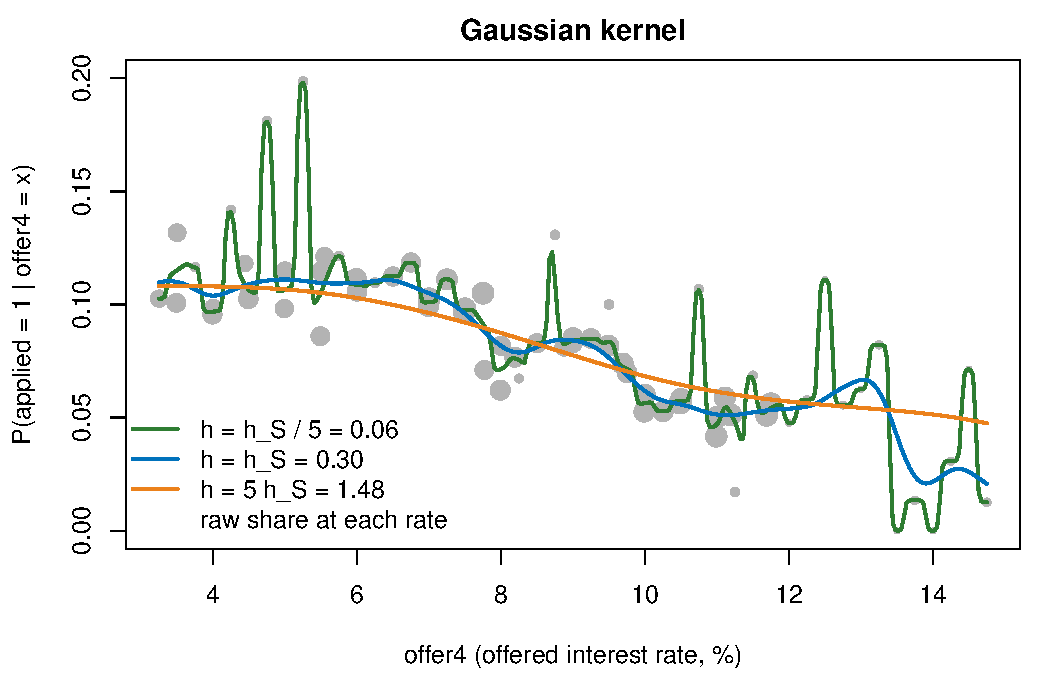
\includegraphics[width=0.75\linewidth]{figures/p3_gaussian.pdf}\\
	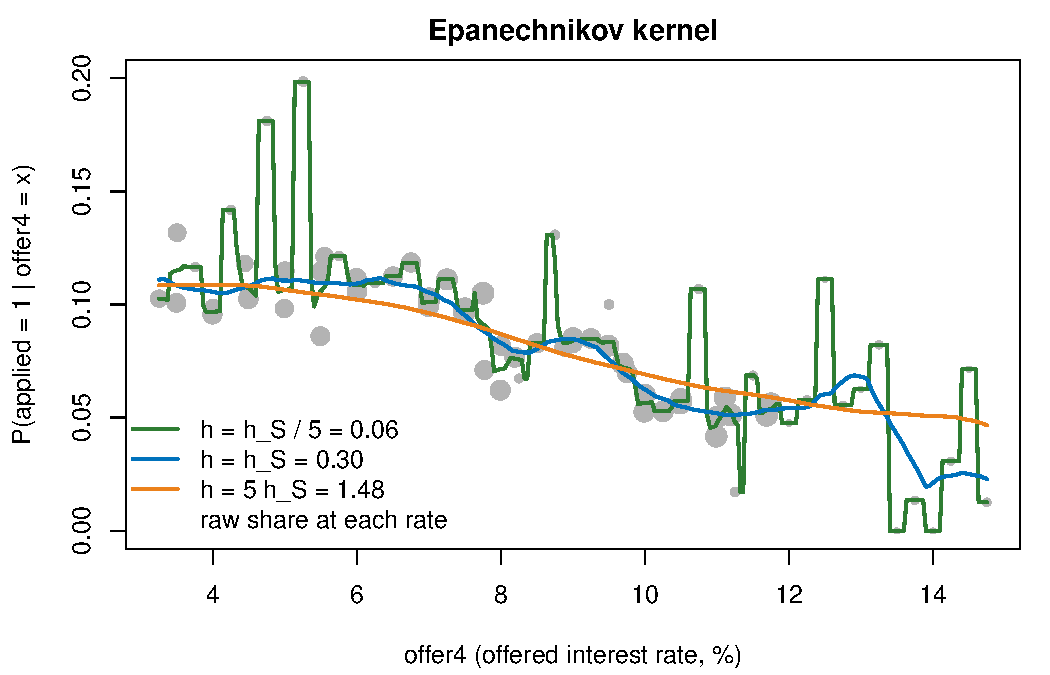
\includegraphics[width=0.75\linewidth]{figures/p3_epanechnikov.pdf}
	\caption{Nadaraya--Watson estimates of $\Prob(\texttt{applied}=1\mid\texttt{offer4}=x)$.}
	\label{fig:p3}
\end{figure}

With Silverman's bandwidth, the application probability falls from about $10.4\%$ at a rate of $4$ to $8.2\%$ at $8$ and $5.4\%$ at $12$: demand slopes down, as in the paper.

\itm{e}
\begin{itemize}
	\item \textbf{The bandwidth matters far more than the kernel.} With $h_S$ the two curves are almost identical (they never differ by more than $0.0055$). With $5h_S$ both are smooth, nearly linear declines.
	\item \textbf{Small bandwidth.} With $h_S/5$ both curves undersmooth: they chase the noise in thinly populated rates (the spikes near $5.25$ and above $12$, where few clients were offered each rate). Here the kernels look different. \texttt{offer4} takes only 70 distinct values, mostly on a grid of $0.25$. The Epanechnikov kernel gives zero weight beyond $\sqrt5\cdot 0.06\approx 0.13$, so at most points it averages only the clients at the nearest rate, and the curve is a sequence of flat steps that jump between rates. The Gaussian kernel never gives zero weight, so its curve moves smoothly from one rate to the next. The differences reach $0.077$.
	\item \textbf{Large bandwidth.} With $5h_S$ the curves are smooth but biased where the true curve bends, and they are pulled toward the interior at the edges of the data (above $14$, the large-$h$ curve stays at about $5\%$ while the data are lower), the boundary bias of the local-constant estimator from Problem 2.
\end{itemize}

\lstinputlisting[caption={Problem 3 (\texttt{code/p3\_karlan.R})}]{code/p3_karlan.R}

%=====================================================================
\problem

Let $X_1,\dots,X_n$ be i.i.d.\ $U[0,\theta]$ and $R_n = n\big(X_{(n)}-\theta\big)$.

\itm{a}
Every $X_i\le\theta$ with probability one, so $X_{(n)}=\max_iX_i\le\theta$ and $R_n\le 0$.

\itm{b}
The maximum is below $t$ if and only if every observation is below $t$, so for $t\in[0,\theta]$, $\Prob(X_{(n)}\le t) = \prod_i\Prob(X_i\le t) = (t/\theta)^n$. Hence
\[
J_n(x,P) = \Prob\left(X_{(n)}\le\theta+\frac xn\right) =
\begin{cases}
0, & x< -n\theta,\\[2pt]
\left(1+\dfrac{x/\theta}{n}\right)^{n}, & -n\theta\le x\le 0,\\[8pt]
1, & x> 0.
\end{cases}
\]
Fix $x\le 0$. For $n$ large, $-n\theta\le x$, and the hint with $r=x/\theta$ gives $J_n(x,P)\to e^{x/\theta}$. For $x>0$, $J_n(x,P)=1$ for all $n$. So $J_n(x,P)\to J(x,P)$ at every $x$, with
\[
J(x,P) = \begin{cases} e^{x/\theta}, & x\le 0\\ 1, & x>0\end{cases}
\;=\; \Prob(-\theta X\le x),\qquad X\sim\mathrm{Exp}(1),
\]
since for $x\le 0$, $\Prob(-\theta X\le x) = \Prob(X\ge -x/\theta) = e^{x/\theta}$. That is, $R_n\xrightarrow{d}-\theta X$.

\itm{c}
Write $\theta_n\equiv\theta(P_n)$ for the largest support point of $P_n$. Since $\varepsilon>0$,
\[
\Prob\Big(n\big(X_{(n),n}-\theta_n\big)\le-\varepsilon\Big) = \Prob\Big(X_{(n),n}\le\theta_n-\frac{\varepsilon}{n}\Big) \le \Prob\big(X_{(n),n}<\theta_n\big).
\]
The sample maximum is below $\theta_n$ if and only if no draw hits the top point $\theta_n$. Each draw hits it with probability $1/n$ (the $n$ points are distinct and equally likely), independently, so
\[
\Prob\big(X_{(n),n}<\theta_n\big) = \left(1-\frac1n\right)^n \longrightarrow e^{-1}
\]
by the hint with $r=-1$. Hence, for every $\varepsilon>0$,
\[
\limsup_{n\to\infty}\Prob\Big(n\big(X_{(n),n}-\theta(P_n)\big)\le-\varepsilon\Big)\le e^{-1}.
\]

\itm{d}
By definition, $J_n(-\varepsilon,P_n) = \Prob\big(n(X_{(n),n}-\theta(P_n))\le-\varepsilon\big)$. Take $0<\varepsilon<\theta$. Then $-\varepsilon/\theta>-1$, and by item c)
\[
\limsup_{n\to\infty} J_n(-\varepsilon,P_n) \le e^{-1} < e^{-\varepsilon/\theta} = J(-\varepsilon,P).
\]
$J(\cdot,P)$ is continuous, so convergence in distribution would require $J_n(x,P_n)\to J(x,P)$ at every $x$. It fails at $x=-\varepsilon$, so $J_n(\cdot,P_n)$ does not converge to $J(\cdot,P)$.

\itm{e}
The bootstrap estimates $J_n(\cdot,P)$ by $J_n(\cdot,\hat P_n)$, where $\hat P_n$ is the empirical distribution. Since $P$ is continuous, the $n$ observations are distinct with probability one, so $\hat P_n$ puts mass $1/n$ on $n$ distinct points of $[0,\theta]$, and $\theta(\hat P_n)=X_{(n)}$. That is, $\hat P_n$ is exactly a distribution of the kind studied in items c) and d), and the argument there applies conditional on the data. The bootstrap root is $R_n^* = n\big(X^*_{(n)}-X_{(n)}\big)$, and items c)--d) show that its distribution does not approach $J(\cdot,P)$. In fact, the bootstrap root equals zero whenever some bootstrap draw hits the sample maximum, so
\[
\Prob^*\big(R_n^*=0\big) = 1-\left(1-\frac1n\right)^n\longrightarrow 1-e^{-1}\approx 0.63,
\]
while the true limit $-\theta X$ has no mass at zero. The bootstrap distribution keeps a large atom at zero; the true distribution never does.

The reason is that bootstrap consistency needs $J_n(\cdot,P_n)\to J(\cdot,P)$ along sequences $P_n\to P$ that include the empirical distribution. The maximum depends on the extreme right tail, exactly where $\hat P_n$ is a poor approximation of $P$: $\hat P_n$ has no mass above $X_{(n)}$ and a mass of $1/n$ at $X_{(n)}$, while $P$ has a density there. Confidence intervals for $\theta$ built from this bootstrap do not have the right coverage, even asymptotically.

%=====================================================================
\problem

\itm{a}
Given $x_i$, the term $\alpha+\beta x_i$ is a constant and $\epsilon_i\mid x_i\sim N(0,2+x_i^2)$, so
\[
y_i\mid x_i\sim N\big(2+5x_i,\ 2+x_i^2\big).
\]
The conditional mean is linear, so OLS is consistent for $(\alpha,\beta)$; the conditional variance grows with $x_i^2$, so the errors are heteroskedastic. We read $x\sim N(0,3)$ as variance $3$.

\itm{b, c}
Figure~\ref{fig:p5} (left) shows one simulated sample of size $n=100$. OLS gives $\hat\alpha = 2.169$ and $\hat\beta = 4.893$. The fanning out of the points as $|x|$ grows is the heteroskedasticity.

\begin{figure}[H]
	\centering
	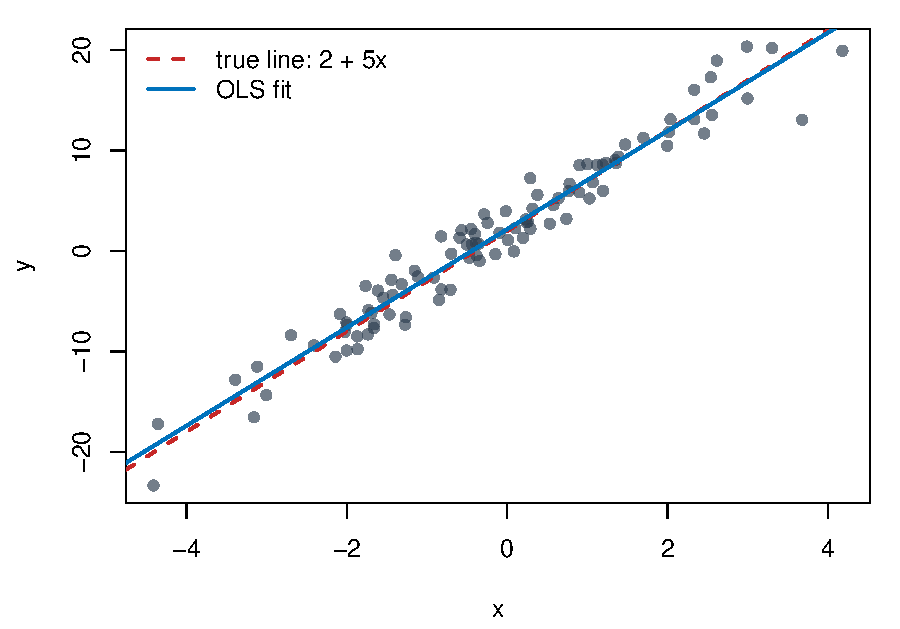
\includegraphics[width=0.49\linewidth]{figures/p5_scatter.pdf}
	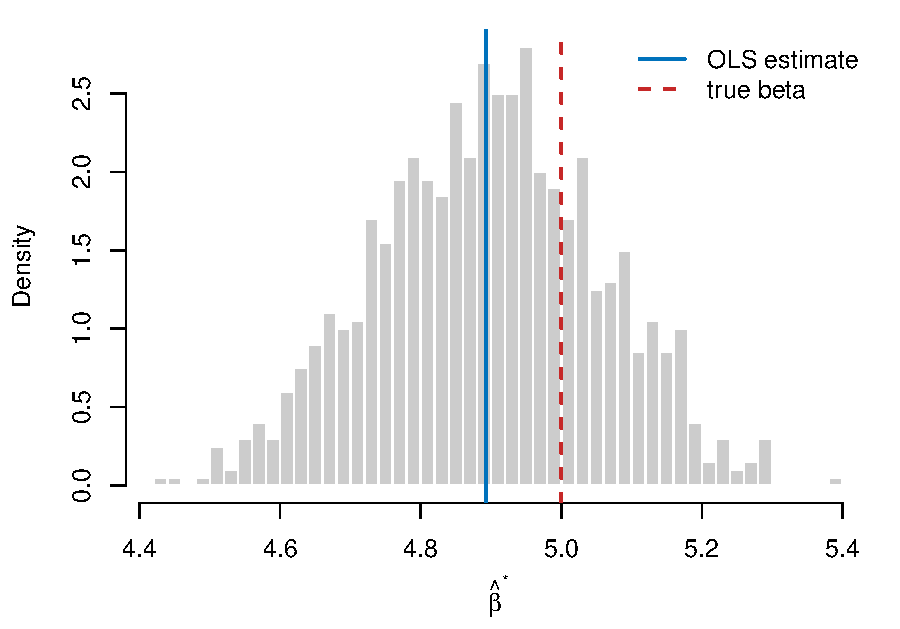
\includegraphics[width=0.49\linewidth]{figures/p5_bootstrap_hist.pdf}
	\caption{Left: one sample with the true line and the OLS fit. Right: the $B=1000$ bootstrap estimates $\hat\beta^*$.}
	\label{fig:p5}
\end{figure}

\itm{d}
The three intervals are $\hat\beta\pm 1.96\cdot\mathrm{se}$:
\begin{itemize}
	\item the usual OLS standard error, $\hat s^2(X'X)^{-1}_{22}$ with $\hat s^2 = \sum\hat\epsilon_i^2/(n-2)$;
	\item the heteroskedasticity-robust (HC1) standard error, from $\frac{n}{n-2}(X'X)^{-1}\big(\sum_i\hat\epsilon_i^2x_ix_i'\big)(X'X)^{-1}$;
	\item the bootstrap standard error: the standard deviation of $\hat\beta^*$ over $B=1000$ pairs-bootstrap samples, each drawing $n$ pairs $(y_i,x_i)$ with replacement. Resampling pairs keeps each error with its own $x_i$, so it keeps the heteroskedasticity.
\end{itemize}

\begin{table}[H]
	\centering
	\begin{tabular}{lccc}
		\toprule
		& Standard error & \multicolumn{2}{c}{95\% confidence interval} \\
		\midrule
		OLS (homoskedastic) & 0.115 & 4.668 & 5.118 \\
		Robust (HC1) & 0.158 & 4.584 & 5.202 \\
		Bootstrap (pairs, $B=1000$) & 0.159 & 4.581 & 5.205 \\
		\bottomrule
	\end{tabular}
\end{table}

The robust and bootstrap standard errors are almost identical, and about $40\%$ larger than the usual one. The histogram of $\hat\beta^*$ in Figure~\ref{fig:p5} (right) is bell shaped and centered at $\hat\beta$, not at $\beta=5$: the bootstrap reproduces the spread of $\hat\beta$, not its location.

\itm{e}
Over $m=500$ simulated samples:

\begin{table}[H]
	\centering
	\begin{tabular}{lcc}
		\toprule
		& Coverage of $\beta=5$ & Average length \\
		\midrule
		OLS (homoskedastic) & 80.6\% & 0.503 \\
		Robust (HC1) & 92.4\% & 0.714 \\
		Bootstrap (pairs) & 93.0\% & 0.708 \\
		\bottomrule
	\end{tabular}
\end{table}

The usual interval is far too short. We can predict its coverage. The true asymptotic variance of $\hat\beta$ is the sandwich
\[
\frac1n\frac{\E[x^2(2+x^2)]}{(\E[x^2])^2} = \frac1n\frac{2\cdot 3+27}{9} = \frac{3.67}{n},
\]
using $\E[x^4]=3\cdot 3^2=27$, while the homoskedastic formula estimates $\frac1n\frac{\E[2+x^2]}{\E[x^2]} = \frac{1.67}{n}$. The usual standard error is too small by a factor $\sqrt{1.67/3.67}=0.67$, so its nominal $95\%$ interval actually covers with probability about $2\Phi(1.96\cdot 0.67)-1\approx 0.81$, which is what we find. The variance of $\epsilon_i$ is largest exactly where $x_i$ is far from its mean, the observations that drive $\hat\beta$, so ignoring heteroskedasticity understates the uncertainty.

The robust and bootstrap intervals both account for heteroskedasticity and cover close to $95\%$. The remaining shortfall is a small-sample effect: with $n=100$, the sandwich is estimated with some downward bias, because the observations with large $|x_i|$ (high leverage) are also the ones with the largest error variance, and OLS residuals at high-leverage points are too small on average. The two methods target the same asymptotic variance, so they perform alike.

\lstinputlisting[caption={Problem 5 (\texttt{code/p5\_ols\_bootstrap.R})}]{code/p5_ols_bootstrap.R}

%=====================================================================
\problem

\itm{a}
The function \texttt{kde\_ci} at the end of this problem does it. Two implementation details are worth noting. First, $h$ is computed once from the original sample and reused in every bootstrap sample. Second, $\hat f_n(x)$ is the sample mean of $k_i = K\big((X_i-x)/h\big)/h$, and with $h$ fixed, resampling the $X_i$'s amounts to resampling the $k_i$'s. So the code computes the $k_i$'s once and each $\hat f^*_{n,b}(x)$ is the mean of $n$ draws, with replacement, from them. This is the same bootstrap, only faster. The interval is
\[
\left[\hat f_n(x)-L_n^{-1}(0.975),\ \hat f_n(x)-L_n^{-1}(0.025)\right].
\]

\itm{b}
With $n=500$, $m=1000$ samples and $B=1000$:

\begin{table}[H]
	\centering
	\begin{tabular}{lccccc}
		\toprule
		& Coverage & Average width & Bias of $\hat f_n(x)$ & s.d.\ of $\hat f_n(x)$ & Bias/s.d. \\
		\midrule
		$x=0$ & 83.2\% & 0.081 & $-0.0168$ & 0.0219 & $-0.77$ \\
		$x=1$ & 94.6\% & 0.071 & $-0.0005$ & 0.0181 & $-0.03$ \\
		\bottomrule
	\end{tabular}
\end{table}

Here $f(0)=0.399$ and $f(1)=0.242$. The bias and s.d.\ columns are computed across the $m$ simulated samples. The interval at $x=1$ has the right coverage; the one at $x=0$ misses $f(0)$ about one time in six.

\itm{c}
For the standard normal, $f'(x)=-x\phi(x)$ and
\[
f''(x) = (x^2-1)\phi(x),\qquad f''(0) = -\phi(0) = -0.399,\qquad f''(1) = 0 .
\]
By Problem 1 e), the bias is about $\frac{h^2}{2}f''(x)$. At $x=0$, the mode, the density is concave and $\hat f_n(0)$ is biased downward; with $h\approx 1.06\cdot 500^{-1/5}=0.31$ the bias is about $-0.019$. (For the Gaussian kernel and normal data there is an exact formula: $\E[\hat f_n(x)]$ is the $N(0,1+h^2)$ density at $x$, which gives $-0.017$, as in the simulation.) This bias is about three quarters of the standard deviation of $\hat f_n(0)$. The interval is built around $\hat f_n(0)$, which is typically too low, so the whole interval is shifted down relative to $f(0)$ and covers less than $95\%$. At $x=1$, an inflection point of $\phi$, the leading bias vanishes, the bias is negligible relative to the standard deviation, and the coverage is close to the nominal level.

\itm{d}
Conditional on the data, each bootstrap draw $X_i^*$ is uniform over $\{X_1,\dots,X_n\}$, so
\[
\E^*\left[\frac1hK\!\left(\frac{X_i^*-x}{h}\right)\right] = \frac1n\sum_{j=1}^n\frac1hK\!\left(\frac{X_j-x}{h}\right) = \hat f_n(x),
\qquad\text{hence}\qquad
\E^*\big[\hat f^*_n(x)\big] = \frac1n\sum_{i=1}^n\hat f_n(x) = \hat f_n(x).
\]
(The same $h$ is used in both, which is why this holds exactly.) So the bootstrap roots $R^*_{n,b}=\hat f^*_{n,b}(x)-\hat f_n(x)$ have mean zero: the bootstrap ``sees'' no bias at all. In the bootstrap world the truth is $\hat f_n(x)$, and $\hat f^*_n(x)$ is unbiased for it. In the real world the truth is $f(x)$, and $\hat f_n(x)$ is unbiased only for the smoothed density $\E[\hat f_n(x)] = \int K(u)f(x+hu)\,du$. The bootstrap gets the variance right but not the bias, so the interval is a valid interval for the smoothed density, not for $f(x)$.

\itm{e}
With $n=2000$ at $x=0$, the coverage is $86.2\%$ (average width $0.050$, bias $-0.0103$, s.d.\ $0.0129$, so bias/s.d.\ $=-0.80$). More data does not fix it: the interval is narrower, but it is still centered in the wrong place. With Silverman's rule, $h\propto n^{-1/5}$, so
\[
\text{bias}\approx\frac{h^2}{2}|f''(0)|\propto n^{-2/5},\qquad
\text{s.d.}\approx\sqrt{\frac{f(0)R(K)}{nh}}\propto n^{-2/5}.
\]
Both shrink at the same rate, so their ratio does not shrink:
\[
\frac{\text{bias}}{\text{s.d.}} \approx \frac{|f''(0)|}{2}\sqrt{\frac{nh^5}{f(0)R(K)}} = \frac{0.399}{2}\sqrt{\frac{1.06^5}{0.399\cdot 0.282}}\approx 0.69,
\]
with $R(\phi)=1/(2\sqrt\pi)=0.282$, whatever $n$ is. A normal approximation then puts the coverage at $\Phi(1.96-0.69)-\Phi(-1.96-0.69)\approx 89\%$ even as $n\to\infty$. In our samples the ratio is a bit larger ($0.77$ and $0.80$) because, with $h\approx 0.3$, the variance still has a non-negligible negative term $-\big(\E[\hat f_n(x)]\big)^2/n$ (see Problem 1 c)), which fades only slowly. So the coverage creeps up from $83\%$ toward about $89\%$, and never reaches $95\%$. This is the role of the condition $nh^5\to 0$ (rather than $nh^5=O(1)$) from the lecture: Silverman's rule is built to minimize mean squared error, which balances squared bias and variance, so the bias stays of the same order as the standard deviation.

\itm{f}
With $h/3$ (same rule, divided by $3$, in the original and the bootstrap samples), at $n=500$ and $x=0$, the coverage is $93.6\%$ and the average width is $0.169$, against $83.2\%$ and $0.081$ with Silverman's $h$ (the bias is $-0.0002$ and the s.d.\ $0.0431$). To leading order, dividing $h$ by $3$ divides the bias by $9$ and multiplies the standard deviation by $\sqrt3\approx 1.73$ (here by $2$, as the negative $O(1/n)$ variance term matters less with a small $h$), so the bias-to-s.d.\ ratio falls by a factor of about $15$, to about $0.05$. The bias becomes negligible and the coverage is back near $95\%$. The price is precision: the interval is about twice as wide, and the estimator has a larger mean squared error (its s.d.\ alone, $0.043$, exceeds the root-MSE with Silverman's $h$, $\sqrt{0.0168^2+0.0219^2}=0.028$). This is the trade-off: a bandwidth that is good for estimation (small MSE) is too large for inference, and valid intervals require undersmoothing, at the cost of wider intervals.

\lstinputlisting[caption={Problem 6 (\texttt{code/p6\_kde\_bootstrap.R})}]{code/p6_kde_bootstrap.R}

%=====================================================================
\clearpage
\section*{Appendix: Consistency of the Local-Linear Estimator}

Lecture 1 states the asymptotic distribution of the local-linear estimator and refers to Hansen's \emph{Econometrics} for the proof, but it does not prove consistency. This appendix does, in two ways. The first is direct: write the estimator as a ratio of kernel averages and show that each average converges, as in Problem 1. The second treats the estimator as an extremum estimator. It uses the same averages, and it shows why the intercept recovers $m(x)$.

\textbf{Setup.} We observe $(Y_i,X_i)$, $i=1,\dots,n$. Let $m(z)=\E[Y\mid X=z]$ and $\mu_2(z)=\E[Y^2\mid X=z]$. Fix a point $x$ and write
\[
u_i = \frac{X_i-x}{h},\qquad K_i = K(u_i),\qquad \kappa_j = \int u^jK(u)\,du,
\]
so $\kappa_0=1$, $\kappa_1=0$ by symmetry, and $\kappa_2>0$ is the kernel's variance. We assume:
\begin{enumerate}[({A}1)]
	\item $(Y_i,X_i)$ are i.i.d.\ with $\E[Y^2]<\infty$. $X$ has a density $f$ with $M=\sup_zf(z)<\infty$; $f$ is continuous at $x$ and $f(x)>0$.
	\item $m$ is continuous at $x$, and $\mu_2(z)f(z)\le C$ for all $z$.
	\item $K$ is a symmetric density, bounded by $\bar K$, with $\int u^4K(u)\,du<\infty$.
	\item $h\to 0$ and $nh\to\infty$.
\end{enumerate}
These are weaker than what the asymptotic distribution needs: no derivatives of $m$ or $f$, and no condition such as $nh^5=O(1)$. The Gaussian and Epanechnikov kernels satisfy (A3). Condition (A2) holds, for example, if $m$ and $\sigma^2(z)=\Var(Y\mid X=z)$ are bounded, since then $\mu_2f\le(\sup m^2+\sup\sigma^2)M$.

\begin{proposition}\label{prop:ll}
Under (A1)--(A4), $m_{LL}(x)\xrightarrow{p}m(x)$.
\end{proposition}

\subsection*{Proof 1: direct}

\emph{Step 1: the estimator as a ratio of kernel averages.} Define, for $j=0,1,2$,
\[
s_j = \frac1n\sum_{i=1}^n\frac1hK_i\,u_i^j,\qquad t_j = \frac1n\sum_{i=1}^n\frac1hK_i\,u_i^jY_i .
\]
Note that $s_0=\hat f_n(x)$ is the kernel density estimator of Problem 1. In the closed form of Problem 2 a), the weights are $K_h(X_i-x)=K_i/h$ and $(X_i-x)^j=h^ju_i^j$, so $S_j=nh^js_j$ and $T_j=nh^jt_j$. Numerator and denominator both pick up the factor $n^2h^2$, which cancels:
\begin{equation}\label{eq:llratio}
m_{LL}(x) = \frac{S_2T_0-S_1T_1}{S_0S_2-S_1^2} = \frac{s_2t_0-s_1t_1}{s_0s_2-s_1^2}.
\end{equation}
(When the denominator is zero the estimator is undefined; give it any value. We show below that this happens with probability going to zero.)

\emph{Step 2: each average converges.}
\begin{lemma}\label{lem:moments}
Under (A1)--(A4), $s_j\xrightarrow{p}\kappa_jf(x)$ for $j=0,1,2$, and $t_j\xrightarrow{p}\kappa_j\,m(x)f(x)$ for $j=0,1$.
\end{lemma}
\begin{proof}
As in Problem 1 d), we show that the mean converges and the variance goes to zero; Chebyshev's inequality then gives convergence in probability.

\emph{The $s_j$'s.} By the change of variables \eqref{eq:cv},
\[
\E[s_j] = \E\left[\frac1hK_iu_i^j\right] = \int K(u)u^jf(x+hu)\,du,
\qquad\text{so}\qquad
\E[s_j]-\kappa_jf(x) = \int K(u)u^j\big[f(x+hu)-f(x)\big]du .
\]
For each $u$ the integrand goes to zero as $h\to 0$, because $f$ is continuous at $x$. It is bounded by $2M|u|^jK(u)\le 2M(1+u^2)K(u)$, which is integrable. By dominated convergence, $\E[s_j]\to\kappa_jf(x)$. For the variance, using independence, $K^2\le\bar KK$, and the same change of variables,
\[
\Var(s_j)\le\frac1n\E\left[\frac1{h^2}K_i^2u_i^{2j}\right] = \frac1{nh}\int K^2(u)u^{2j}f(x+hu)\,du \le \frac{M\bar K}{nh}\int(1+u^4)K(u)\,du\ \longrightarrow\ 0,
\]
since $nh\to\infty$.

\emph{The $t_j$'s.} Let $g(z)=m(z)f(z)$. By the law of iterated expectations, $\E[K_iu_i^jY_i\mid X_i]=K_iu_i^jm(X_i)$, so
\[
\E[t_j] = \E\left[\frac1hK_iu_i^jm(X_i)\right] = \int K(u)u^jg(x+hu)\,du .
\]
The function $g$ is continuous at $x$, as a product of functions continuous at $x$. It is also bounded: by Jensen's inequality $m(z)^2\le\mu_2(z)$, so $|g(z)|\le\sqrt{\mu_2(z)f(z)}\,\sqrt{f(z)}\le\sqrt{CM}$. The dominated convergence argument used for $s_j$ then gives $\E[t_j]\to\kappa_jg(x)$. For the variance, iterated expectations again turn $Y_i^2$ into $\mu_2(X_i)$:
\begin{align*}
\Var(t_j)\le\frac1n\E\left[\frac1{h^2}K_i^2u_i^{2j}\mu_2(X_i)\right] &= \frac1{nh}\int K^2(u)u^{2j}\mu_2(x+hu)f(x+hu)\,du\\
&\le\frac{C\bar K}{nh}\int(1+u^2)K(u)\,du\ \longrightarrow\ 0. \qedhere
\end{align*}
\end{proof}

\emph{Step 3: the ratio converges.} By Lemma~\ref{lem:moments} and the continuous mapping theorem,
\[
s_0s_2-s_1^2\xrightarrow{p}\kappa_2f(x)^2,\qquad s_2t_0-s_1t_1\xrightarrow{p}\kappa_2f(x)\cdot m(x)f(x)-0 = \kappa_2\,m(x)f(x)^2 .
\]
The limit of the denominator is strictly positive, since $\kappa_2>0$ and $f(x)>0$. So the probability that the denominator is positive (that is, that $Z'W^{-1}Z$ in Problem 2 a) is invertible) goes to one. The map $(a,b)\mapsto a/b$ is continuous wherever $b\neq 0$, so by the continuous mapping theorem and \eqref{eq:llratio},
\[
m_{LL}(x)\xrightarrow{p}\frac{\kappa_2\,m(x)f(x)^2}{\kappa_2f(x)^2} = m(x). \qquad\qed
\]

\emph{What drives the result.} The key step is $s_1\xrightarrow{p}0$. In the limit, the matrix $\begin{pmatrix}s_0&s_1\\ s_1&s_2\end{pmatrix}$ (which is $Z'W^{-1}Z$, rescaled) becomes $f(x)\,\mathrm{diag}(1,\kappa_2)$. It is diagonal because a symmetric kernel puts as much weight to the left of $x$ as to the right, so the local regressor $u_i$ is uncorrelated with the constant. Then the intercept no longer depends on the slope, and \eqref{eq:llratio} reduces to $t_0/s_0$, the Nadaraya--Watson estimator, whose limit is $g(x)/f(x)=m(x)$. In finite samples $s_1\neq 0$, and the slope correction is what removes the design bias discussed in Problem 2 d). It does not matter for consistency.

\subsection*{Proof 2: as an extremum estimator}

Lecture 1 defines $m_{LL}(x)$ as the minimizer of a weighted least-squares criterion, so it is an extremum estimator. To use the consistency theorem for extremum estimators, we need a criterion with a non-degenerate limit, which takes two adjustments, since the criterion changes with $n$ through $h$:
\begin{enumerate}[(i)]
	\item \emph{Divide by $nh$.} Only a share of about $2hf(x)$ of the observations gets non-negligible weight, so the average of the weighted squared residuals goes to zero. Dividing by $nh$ instead of $n$ keeps it of order one.
	\item \emph{Measure the slope in units of the bandwidth.} Over a window of width $h$, a line with slope $b_1$ rises by about $hb_1$. That is the quantity the local data can pin down, so we write $c=hb_1$ and $b_1(X_i-x)=c\,u_i$.
\end{enumerate}
The criterion is then
\[
Q_n(a,c) = \frac1{nh}\sum_{i=1}^nK_i\big(Y_i-a-c\,u_i\big)^2 .
\]
It is the lecture's criterion divided by $nh$, with the slope reparametrized. So its minimizer is $a=m_{LL}(x)$ and $c=h\,m'_{LL}(x)$, where $m'_{LL}(x)$ is the estimated local slope. Expanding the square,
\[
Q_n(a,c) = A_n - 2a\,t_0 - 2c\,t_1 + a^2s_0 + 2ac\,s_1 + c^2s_2,\qquad A_n=\frac1{nh}\sum_{i=1}^nK_iY_i^2 .
\]
The term $A_n$ does not depend on $(a,c)$, so we drop it: $\tilde Q_n=Q_n-A_n$ has the same minimizer. (This also saves us from assuming anything about the limit of $A_n$.) For each fixed $(a,c)$, $\tilde Q_n(a,c)$ is a fixed linear combination of the $s_j$'s and $t_j$'s, so Lemma~\ref{lem:moments} gives
\[
\tilde Q_n(a,c)\xrightarrow{p}\tilde Q(a,c) = f(x)\Big[a^2+\kappa_2c^2-2a\,m(x)\Big] = f(x)\Big[\big(a-m(x)\big)^2+\kappa_2c^2-m(x)^2\Big].
\]
Since $f(x)>0$ and $\kappa_2>0$, the limit $\tilde Q$ has a unique minimum at $(a,c)=(m(x),0)$.

The usual consistency theorem for extremum estimators needs a compact parameter space and uniform convergence of the criterion. Neither holds here: the parameter space is $\mathbb R^2$, and we only have convergence at each point. Convexity makes up for both. The following is the minimization version of Theorem 2.7 in Newey and McFadden (1994).\footnote{W.~K.~Newey and D.~McFadden (1994), ``Large Sample Estimation and Hypothesis Testing,'' in R.~F.~Engle and D.~L.~McFadden (eds.), \emph{Handbook of Econometrics}, Vol.~4, Ch.~36.}

\begin{nmtheorem}
Suppose that (i) $Q_0(\theta)$ is uniquely minimized at $\theta_0$; (ii) $\theta_0$ is in the interior of a convex set $\Theta$ and $\hat Q_n(\theta)$ is convex on $\Theta$; and (iii) $\hat Q_n(\theta)\xrightarrow{p}Q_0(\theta)$ for every $\theta\in\Theta$. Then, with probability going to one, $\hat Q_n$ has a minimizer $\hat\theta$ on $\Theta$, and $\hat\theta\xrightarrow{p}\theta_0$.
\end{nmtheorem}

Take $\Theta=\mathbb R^2$, $\hat Q_n=\tilde Q_n$, $Q_0=\tilde Q$ and $\theta_0=(m(x),0)$. Condition (i) was shown above. For (ii), $\tilde Q_n$ is a sum of squares with nonnegative weights, minus a constant, so it is convex. Condition (iii) is the pointwise limit above. Hence
\[
m_{LL}(x)\xrightarrow{p}m(x)\qquad\text{and}\qquad h\,m'_{LL}(x)\xrightarrow{p}0 .
\]

\emph{Two remarks.} First, the two proofs do the same computation in a different order. Proof~1 minimizes first (the closed form) and then takes the limit; Proof~2 takes the limit of the criterion first and then minimizes. They agree because the criterion is quadratic. Second, $h\,m'_{LL}(x)\xrightarrow{p}0$ says nothing about the slope estimate itself. In the limit criterion the slope enters only through $\kappa_2c^2$, which is minimized at $c=0$ whatever $m'(x)$ is: at the scale of the bandwidth, every smooth function looks flat. Estimating $m'(x)$ consistently needs a finer argument and a stronger condition on $h$ (the variance of $m'_{LL}(x)$ is of order $1/(nh^3)$, not $1/(nh)$), which we do not pursue here.

\end{document}
